\documentclass[preprint,12pt,number,sort&compress]{elsarticle}

\usepackage{amsmath,amssymb,amsfonts}
\usepackage{xcolor}
\usepackage{graphicx}
\usepackage{booktabs}
\usepackage{multirow}
\usepackage{makecell}
\usepackage{threeparttable}
\usepackage{tabularx}
\usepackage{longtable}
\usepackage{float}
\usepackage{array}
\usepackage{url}
\usepackage{xurl}
\usepackage{indentfirst}
\usepackage{hyperref}

\emergencystretch=3em
\makeatletter
\pdfstringdefDisableCommands{%
    \def\corref#1{}%
    \def\cnotenum#1{}%
    \def\@corref#1{}%
}
\makeatother

\journal{Reliability Engineering \& System Safety}

\begin{document}

\begin{frontmatter}

\title{CET-STGL: A Causal-Inspired Event-Token Spatio-Temporal Framework for Alarm-Aware KPI Degradation Prediction in Cellular Networks}

\author[tsinghua]{Dun Li\corref{cor1}}
\ead{lidun.2023@tsinghua.org.cn}

\author[tsinghua]{RuoShi Liu}
\ead{liurs23@mails.tsinghua.edu.cn}

\author[polyu]{Ming Li}
\ead{ming.li@polyu.edu.hk}
\ead[url]{https://orcid.org/0000-0003-4119-7340}

\author[tsinghua]{Ruiguan Lin}
\ead{linruiguan@mail.tsinghua.edu.cn}
\ead[url]{https://orcid.org/0000-0003-2035-3770}

\author[crc,polimi]{Enrico Zio}
\ead{enrico.zio@polimi.it}

\cortext[cor1]{Corresponding author.}

\affiliation[tsinghua]{
    organization={Department of Industrial Engineering, Tsinghua University},
    city={Beijing},
    postcode={100084},
    country={China}
}

\affiliation[polyu]{
    organization={Research Institute for Advanced Manufacturing, The Hong Kong Polytechnic University},
    city={Hung Hom},
    country={Hong Kong SAR, China}
}

\affiliation[crc]{
    organization={Center for research on Risk and Crises (CRC), Mines Paris, PSL},
    country={France}
}

\affiliation[polimi]{
    organization={Energy Department, Politecnico di Milano},
    city={Milano},
    country={Italy}
}

\begin{abstract}
Cellular network reliability is monitored through heterogeneous time-evolving telemetry, including key performance indicator (KPI) measurements, business counters, sparse alarm/fault events, anonymized cell identifiers and temporal context. Predicting future KPI degradation is difficult because alarms are sparse, KPI responses may be delayed, physical topology is often unavailable and expert-confirmed fault labels are not always recorded. We study an anonymized real-world mobile broadband (MBB) operations dataset provided by Huawei Technologies. The source collection covers approximately 500 cellular sites, while the aligned panel evaluated in this study contains 33 anonymized cell entities without geographically identifiable site information. We propose CET-STGL, a causal-inspired event-token spatio-temporal framework that combines KPI patches, alarm events, cell/time context, train-only event influence priors and inferred cross-cell context. A lightweight sklearn-based instantiation is evaluated under a leakage-controlled protocol for multi-horizon KPI forecasting, weak degradation classification and weak alarm-candidate prioritization. Results indicate that KPI-history baselines remain strong, standalone event-only predictors are weak, and the evaluated CET-STGL instantiation is competitive on several primary-KPI forecasting metrics. Alarm and graph features show limited and non-uniform aggregate forecasting gains; weak alarm-candidate ranking is interpreted only as proxy consistency, not expert-confirmed fault localization.
\end{abstract}

\begin{highlights}
\item Private cellular KPI/alarm telemetry is studied under leakage-controlled forecasting.
\item CET-STGL organizes KPI patches, sparse alarms, cell/time context and inferred cross-cell context.
\item Forecasting, weak degradation classification and weak alarm-candidate prioritization are evaluated.
\item Reported evidence is limited to runnable lightweight instantiations and weak labels.
\end{highlights}

\begin{keyword}
Cellular network reliability \sep KPI forecasting \sep Alarm correlation \sep Weak alarm-candidate prioritization \sep Spatio-temporal framework \sep Causal-inspired event influence
\end{keyword}

\end{frontmatter}

\section{Introduction}

Cellular network reliability is increasingly managed through structured operational telemetry rather than isolated counters. A cell-level operations panel may contain continuous key performance indicator (KPI) and business counters, sparse alarm/fault events, anonymized cell identifiers, and time context. KPI histories describe load, accessibility, retainability, throughput and radio-quality dynamics; alarms mark discrete operational events; cell and time features encode persistent local behavior and periodic demand. Anticipatory mobile networking has shown that prediction can support proactive resource management \cite{bui2017anticipatory}. Deep-learning studies in mobile networks further connect traffic and performance prediction with data-driven control \cite{zhang2019deepmobile}. Recent O-RAN work stresses explainable, programmable radio access automation \cite{brik2025xaioran}, and mobile-traffic prediction studies show that cross-service correlations can carry useful forecasting information \cite{feng2024multiservice}. For cellular operations, proactive KPI degradation prediction is a reliability problem: the goal is to recognize deteriorating cell conditions before they become service-impacting events or costly manual troubleshooting cases.

The modeling difficulty lies in the heterogeneous form and uneven reliability of the available signals. KPI-history models can exploit strong temporal regularities, yet sparse event context is often part of the evidence that operators inspect during fault handling. Alarm/event models alone are also insufficient for continuous KPI prediction because alarms are rare and many KPI changes follow routine traffic or radio patterns rather than explicit faults. Prior cellular traffic work has emphasized spatial and temporal dependencies among base stations \cite{wang2017spatiotemporal}, while recent mobile traffic forecasting studies show the importance of network-wide temporal patterns \cite{sun2022mobiletraffic}. Classic alarm-correlation work has long noted that a single fault may generate many related alarms \cite{jakobson1993alarm}; communication-network fault-identification studies also show that alarm floods complicate localization \cite{bouloutas1994alarm}. Enterprise operations data add further constraints: physical topology may be unavailable, expert root-cause annotations may be absent, and data release may be restricted by business and network-operation confidentiality.

This paper studies alarm-aware KPI degradation prediction using an anonymized real-world mobile broadband (MBB) operations dataset provided by Huawei Technologies. The source collection covers approximately 500 cellular sites, while the aligned panel evaluated in this study contains 33 anonymized cell entities without geographically identifiable site information. We propose CET-STGL as a causal-inspired event-token spatio-temporal framework for this setting. The central methodological idea is a temporally admissible representation of heterogeneous cellular telemetry: KPI histories are transformed into local patch features, alarms are represented through sparse event and intensity features, and alarm-degradation associations are incorporated as train-only event influence priors. When physical topology is unavailable, cross-cell context is inferred from training-period operational correlations. CET-STGL organizes operational signals under realistic monitoring constraints, without treating observed associations as causal evidence or expert-verified fault localization.
The reliability-oriented pipeline and the main guardrails used throughout the paper are summarized in Fig.~\ref{fig:cet_stgl_overview}.

\begin{figure}[!t]
    \centering
    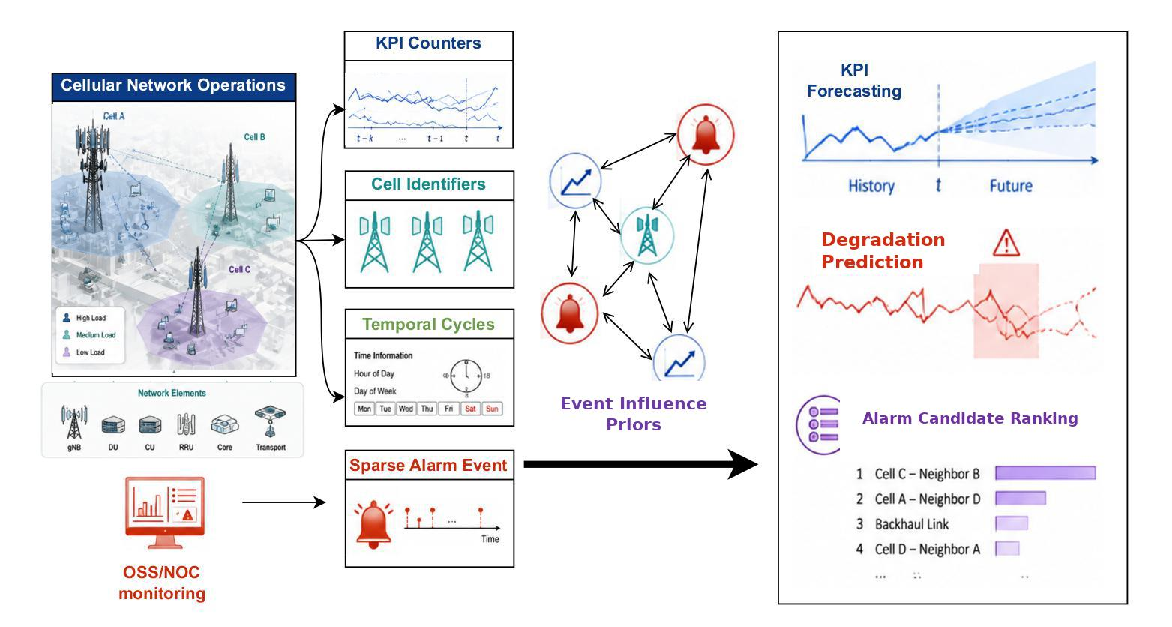
\includegraphics[width=0.98\textwidth]{figures/Fig0_cet_stgl_reliability_overview.pdf}
    \caption{Overview of CET-STGL from reliability-oriented cellular network operations to analysis.}
    \label{fig:cet_stgl_overview}
\end{figure}

Recent telecom LLM discussions examine language models for telecommunications \cite{maatouk2025llmtelecom}. Domain-adapted telecom LLMs focus on language and standards knowledge \cite{zou2025telecomgpt}, and networking LLM systems study adaptation to networking tasks \cite{wu2024netllm}. Benchmark proposals for industrial telecom workflows provide a separate line of context \cite{xiao2026telecombench}. This paper instead works with structured telemetry for cellular reliability analysis, with KPI forecasting, weak degradation classification and weak alarm-candidate prioritization evaluated on a private operations slice. Section~\ref{sec:limitations_reproducibility} states the limits on causality, expert RCA validation and end-to-end neural spatio-temporal graph evaluation.

The paper makes four contributions:
\begin{enumerate}
    \item Alarm-aware KPI degradation prediction is formulated as a multi-task evaluation problem over real cellular KPI/business and alarm/fault panels.
    \item A temporally admissible, causal-inspired event-token representation is formalised that aligns KPI patch features, alarm event features, cell/time context, train-only event influence priors and inferred cross-cell context.
    \item A leakage-controlled reliability evaluation protocol is provided for 1/3/6/12-hour KPI forecasting, weak degradation classification and weak alarm-candidate prioritization.
    \item The empirical findings are narrow by design: KPI-history baselines remain strong, event-intensity variants are weak standalone predictors, the evaluated lightweight CET-STGL instantiation is competitive on several primary-KPI forecasting metrics, and gains from alarm and graph features are limited and non-uniform under the current weak-label protocol.
\end{enumerate}

The remainder of this paper is organized as follows. Section~\ref{sec:related_work} reviews related work. Section~\ref{sec:problem_method} formulates the tasks. Section~\ref{sec:methodology} presents CET-STGL. Section~\ref{sec:experimental_evaluation} reports the experimental evaluation and limitations. Section~\ref{sec:conclusion} concludes the paper.

\section{Related Work}
\label{sec:related_work}

\subsection{Cellular KPI Forecasting and Time-Series Prediction}

Mobile and wireless networking research has studied prediction as a foundation for proactive management. Recent sixth-generation (6G) surveys emphasize programmable, data-driven radio access networks for telemetry-driven control and assurance \cite{wang2023road6g}. O-RAN studies connect radio access programmability with operational automation \cite{polese2023oran}. Recent RAN alarm prediction work reflects the value of modeling sparse alarms with network context \cite{li2025ranalarm}. Universal mobile-traffic forecasting similarly motivates learning cellular traffic dynamics \cite{chai2025uomo}.

General time-series forecasting now spans recurrent, convolutional, transformer, decomposition and language-model-inspired designs. TimesNet represents a recent temporal-variation modeling direction \cite{wu2023timesnet}, while strong linear baselines question whether transformer complexity is always necessary \cite{zeng2023transformers}. Follow-up models explore inverted transformer structures, multiscale mixing and probabilistic sequence pretraining \cite{liu2024itransformer,wang2024timemixer,ansari2024chronos}. Time-LLM and GPT4MTS adapt language-model ideas to time-series prediction \cite{jin2024timellm,jia2024gpt4mts}. Donut and OmniAnomaly further motivate learning from seasonal or multivariate KPI time series in production systems \cite{xu2018donut,su2019omni}. Cellular KPI forecasting studies mainly focus on traffic prediction or individual KPI modeling, whereas operational degradation prediction requires continuous KPI evolution, sparse fault events and cross-cell context. Existing approaches rarely address alarm-KPI coupling under enterprise monitoring conditions with incomplete topology information and expert RCA annotations. CET-STGL addresses this setting by integrating KPI forecasting, weak degradation estimation and alarm-candidate prioritization within an event-token representation framework.

\subsection{Alarm Correlation, RCA and Event Influence Modeling}

Alarm correlation is a classic fault-management problem in communication networks. Recent work has explored alarm-correlation rule mining for network fault management \cite{fournierViger2021alarmrules}, whereas log-based operational diagnosis methods such as DeepLog illustrate the broader role of event sequences in detecting and diagnosing operational anomalies \cite{du2017deeplog}.

Recent artificial intelligence for information technology operations (AIOps) and microservice RCA studies provide methodological background for multimodal observability and graph-based diagnosis. Nezha models multi-modal observability for interpretable root-cause analysis \cite{yu2023nezha}. CausalRCA and neural Granger causal discovery explore causal-inference-inspired localization \cite{xin2023causalrca,lin2024run}, and Chain-of-Event learns weighted event causal graphs for microservice incidents \cite{yao2024chainofevent}. RCAEval and AIOpsLab highlight the need for reproducible RCA evaluation infrastructure \cite{pham2025rcaeval,ma2025aiopslab}. Point-process analysis provides a foundation for self-exciting event sequences \cite{ogata1988pointprocess}, and Hawkes-based Granger modeling connects event intensity with temporal influence estimation \cite{xu2016grangerhawkes}. Existing alarm correlation and RCA methods often focus on post-incident localization. Proactive degradation prediction instead asks whether sparse alarms add useful context before KPI deterioration. In cellular operations, alarms are often noisy, delayed or incomplete, making direct event-based prediction challenging. CET-STGL treats alarms as contextual event signals and studies their contribution through event tokens, temporal intensity and influence modeling. Ranking results are interpreted as weak-label consistency rather than validated RCA, and event influence features are causal-inspired association priors rather than proof of causality.

\subsection{Spatio-Temporal Modeling and Telecom LLM Context}

Spatio-temporal graph neural networks model temporal dynamics and entity dependencies. Recent traffic-forecasting work has developed delay-aware transformers for long-range propagation effects \cite{jiang2023pdformer}. Adaptive spatio-temporal embeddings and large-scale traffic datasets support systematic evaluation of interacting entities \cite{liu2023staeformer,liu2023largest}. Recent KDD work on asynchronous spatio-temporal graph convolution also highlights irregular temporal structure in graph-based forecasting \cite{zhang2024aseer}. Existing spatio-temporal graph learning methods show the importance of interactions among network entities, but cellular degradation prediction remains limited by incomplete topology information and operational labels. CET-STGL adapts this idea to cellular monitoring by using inferred cross-cell context and train-only event influence priors. We evaluate a lightweight sklearn-based instantiation; end-to-end neural graph encoders are left for future evaluation under the same protocol.

Recent telecom and networking LLM work examines language models for standards knowledge, networking tasks and domain adaptation. TeleQnA evaluates whether LLMs capture domain-specific standards and networking concepts \cite{maatouk2026teleqna}. LLM-oriented telecom research helps position telecom-domain AI, but CET-STGL addresses a different data modality: structured operational telemetry for KPI forecasting, weak degradation classification and weak alarm-candidate prioritization on a private operations slice.

\section{Problem Formulation and Methodology}
\label{sec:problem_method}
\label{sec:problem_formulation}

Let $\mathcal{C}$ be the set of cells and let $t$ index hourly timestamps. For each cell-time pair $(c,t)$, the panel contains a KPI/business vector $\mathbf{x}_{c,t}\in\mathbb{R}^{M}$, an alarm/fault vector $\mathbf{a}_{c,t}\in\mathbb{R}^{A}$, an anonymized cell identifier and timestamp-derived features. In the evaluated anonymized MBB operations panel, $|\mathcal{C}|=33$, $M=48$ and $A=137$, although only 11 alarm/fault columns are active in the observed slice. Given a lookback window $\mathcal{W}_{c,t}=\{(\mathbf{x}_{c,\tau},\mathbf{a}_{c,\tau}):t-L+1\leq \tau\leq t\}$, the objective is to predict outcomes at horizon $h\in\{1,3,6,12\}$ hours. Windows crossing the detected long time gap are removed before modeling.

A feature representation for target $(c,t+h)$ is called temporally admissible if it is constructed only from $\mathcal{W}_{c,t}$, static or timestamp-derived identifiers available at $t$, and statistics fitted on the chronological training partition. CET-STGL uses this constraint throughout to separate operationally available evidence from future outcomes.

\subsection{KPI Forecasting}
The forecasting task is to predict future KPI values, as formalized here below:
\begin{equation}
    \hat{\mathbf{x}}_{c,t+h} = f_h(\mathcal{W}_{c,t}, c, t),
\end{equation}
where $\hat{\mathbf{x}}_{c,t+h}$ is the predicted KPI vector at horizon $h$, $\mathcal{W}_{c,t}$ is the historical lookback window for cell $c$ at time $t$, and $f_h$ represents the forecasting mapping function. Forecasting labels are real future observations from the private cellular panel. We report aggregate metrics over all KPI/business columns and paper-level metrics over the primary KPI subset.

\subsection{Weak Degradation Classification}
The degradation task is to predict a weak binary label, formalized as follows:
\begin{equation}
    \hat{y}_{c,t+h} = g_h(\mathcal{W}_{c,t}, c, t), \quad y_{c,t+h}\in\{0,1\},
\end{equation}
where $\hat{y}_{c,t+h}$ is the predicted degradation probability, $y_{c,t+h}$ is the weak binary indicator, and $g_h$ denotes the classification function. The label is derived from thresholds fitted on the training split. The evaluated implementation uses five independent OR conditions: high call-drop rate above the larger of 1.0\% and the cell-specific training 99th percentile; low Radio Resource Control (RRC) setup success rate below the smaller of 98.0\% and the cell-specific training 5th percentile; low Evolved Radio Access Bearer (E-RAB) setup success rate below the smaller of 98.0\% and the cell-specific training 5th percentile; low downlink user throughput in Mbps below the cell-specific training 10th percentile; or low dimensionless Channel Quality Indicator (CQI) below the cell-specific training 10th percentile. Cell-specific thresholds are replaced by the corresponding full-training-partition thresholds when fewer than 24 non-missing training samples are available for the relevant cell and KPI, or when the computed cell-level threshold is not finite. The label is therefore a weak KPI degradation proxy rather than an expert incident label, following weak-supervision practice for indirect or noisy supervision \cite{zhou2018weakly,ratner2020snorkel}.

\subsection{Weak Alarm-Candidate Prioritization}
For degraded samples with recent alarms, the ranking task scores candidate alarm types $a\in\mathcal{A}_{c,t}$ as follows:
\begin{equation}
    s_h(a,c,t)=r_h(a,\mathcal{W}_{c,t},c,t),
\end{equation}
where $s_h(a,c,t)$ is the prioritization score assigned to alarm candidate $a$ in cell $c$ at time $t$, and $r_h$ is the scoring function. The target candidate is induced by train-only alarm-to-degradation lift and recent event intensity. The ranking task evaluates weak-label consistency only. It is not expert-confirmed root-cause localization.

\subsection{Causal-Inspired Graph Boundary}
The event influence graph is constructed from temporal precedence and train-only association. It is useful for organizing candidate event influence, but the observational data contain no interventions or expert causal annotations. We therefore use only causal-inspired terminology and avoid causal-effect claims.

\subsection{CET-STGL Representation and Evaluated Instantiation}
\label{sec:methodology}

\subsubsection{Overview}
CET-STGL is a causal-inspired event-token spatio-temporal representation framework for structured cellular operations data. It contains five feature blocks: KPI patch features, alarm event features, cell/time positional features, an event influence prior and inferred cross-cell context. Representation construction is separated from the downstream learner: heterogeneous signals are first aligned to the same cell-time-horizon index and then passed to forecasting, classification or prioritization heads. We evaluate a lightweight sklearn-based instantiation to isolate the utility of KPI patching, sparse event encoding, temporal context, train-only influence priors and inferred cross-cell information under a leakage-controlled protocol.

\noindent\textbf{Reliability-oriented representation principle.}
The design follows three constraints. KPI histories are summarized as local level and slope patches, sparse alarms are encoded by counts, decayed intensity and train-only association priors, and cross-cell context is inferred from training-period operational correlations when topology is unavailable. Compared with simple feature concatenation, CET-STGL imposes an explicit prediction-time constraint on each $(c,t,h)$ target, treats alarms as temporally weighted event context rather than raw indicators, and uses one admissible cell-time representation across forecasting, weak degradation classification and weak alarm-candidate prioritization.

\noindent\textbf{Temporal admissibility.}
For any prediction target at $(c,t+h)$, the evaluated CET-STGL feature vector is a function only of the lookback window $\mathcal{W}_{c,t}$, identifiers and time features available at $t$, and statistics fitted on the chronological training partition. No validation/test labels, post-$t$ observations or future event information are used in feature construction.

\noindent\textit{Justification.}
KPI patch features, alarm counts and decayed intensities are computed within $\mathcal{W}_{c,t}$. Degradation thresholds, feature scalers, event lifts and cross-cell graph statistics are estimated from the training partition only, and windows crossing the long time discontinuity are excluded before model fitting. The admissibility statement therefore concerns leakage-controlled representation construction, not causal identification or performance optimality.

The model structure and the evaluated lightweight implementation are summarized in Fig.~\ref{fig:cet_stgl_architecture}.

\begin{figure}[!t]
    \centering
    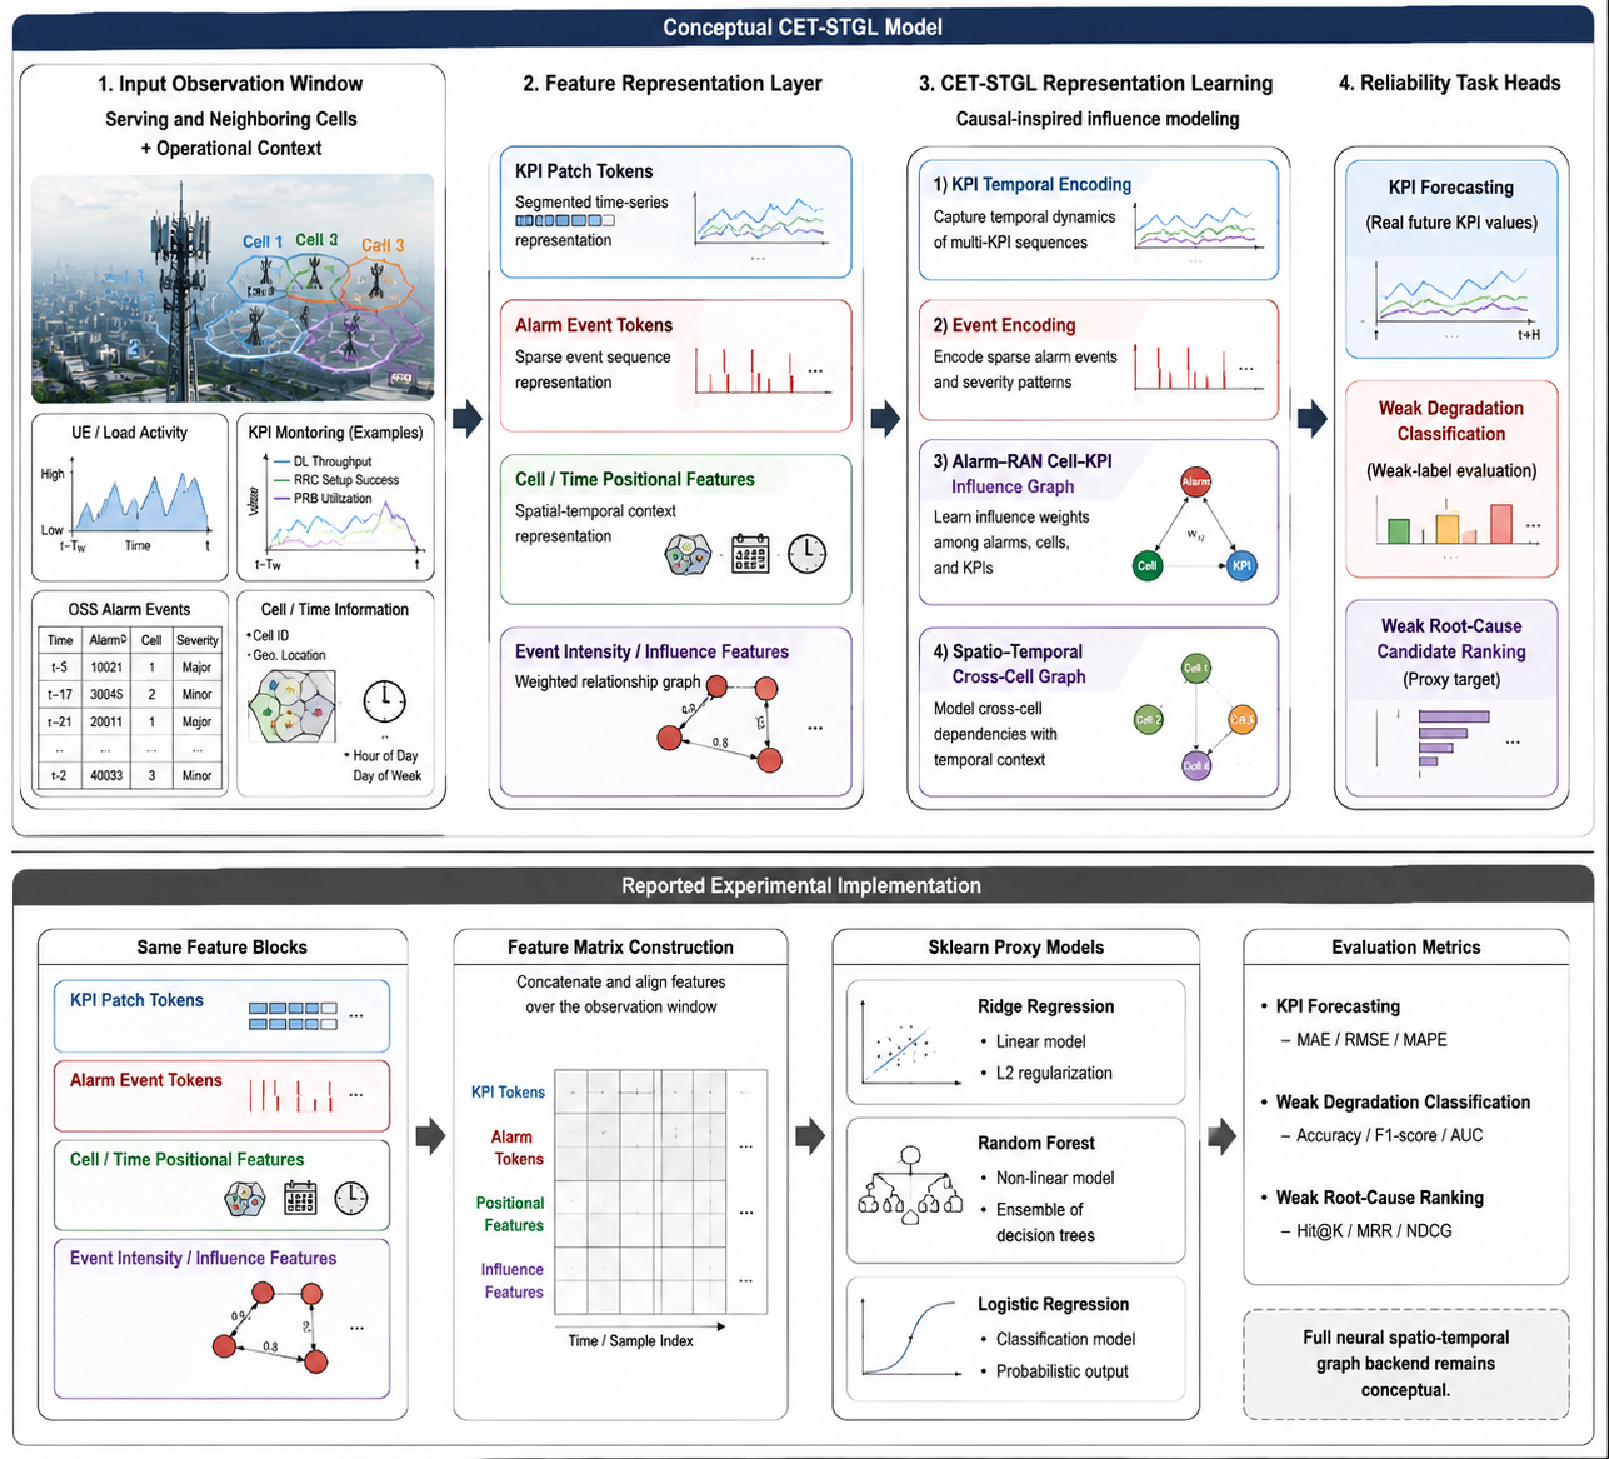
\includegraphics[width=0.98\textwidth]{figures/Fig_cet_stgl_model_architecture.pdf}
    \caption{Conceptual structure of CET-STGL, transforming heterogeneous cellular telemetry into event-aware spatio-temporal representations with influence modeling and a lightweight sklearn-based implementation for evaluation.}
    \label{fig:cet_stgl_architecture}
\end{figure}

\subsubsection{KPI Patch Features}
For each KPI $m$ in a lookback window, the sequence $x^{(m)}_{c,t-L+1:t}$ is divided into short patches. Each patch is summarized by simple local statistics:
\begin{equation}
    \phi^{\mathrm{kpi}}_{c,t,p,m}=
    [\mathrm{mean},\mathrm{slope}]_{c,t,p,m}.
\end{equation}
The patch summaries preserve local temporal level and slope while reducing raw sequence length. Patch-based features also support the multi-column KPI/business schema because all KPI columns can be transformed through the same compact local temporal summarization rule.
Patch-based time-series modeling provides a direct precedent for representing long temporal windows through compact local segments \cite{nie2023patchtst}.

\subsubsection{Alarm Event and Intensity Features}
Alarm/fault observations are represented as sparse event features. For alarm type $a$, we compute rolling counts and a decayed event intensity
\begin{equation}
    \lambda_a(c,t)=\sum_{\tau \leq t} \mathbf{1}[a_{c,\tau}>0]\exp\left(-\frac{t-\tau}{\eta}\right),
\end{equation}
where $\lambda_a(c,t)$ is the decayed event intensity for alarm type $a$ at cell $c$ and time $t$, $\mathbf{1}[a_{c,\tau}>0]$ is the binary indicator of the active alarm event at time $\tau$, and $\eta$ is a fixed decay scale in the feature implementation. The term Hawkes-inspired refers to the recency-weighted form, in which recent events contribute more strongly than older events \cite{hawkes1971spectra,mei2017neuralhawkes}. In the evaluated implementation, the decayed intensity is used as a fixed event feature rather than a fitted multi-type point-process model. Fixed decayed intensity matches the observed alarm sparsity: only 11 of 137 alarm/fault columns are active and only 1.62\% of rows contain an active alarm.

\subsubsection{Cell and Time Positional Features}
Cell identity and time context are encoded through cell-code features and cyclical time features such as hour-of-day and day-of-week. Cell and time positional features capture persistent cell offsets and periodic operational behavior. All transformations are fitted within the chronological training protocol, and windows crossing the detected long time gap are excluded.

\subsubsection{Train-Only Event Influence Prior}
For each alarm type and horizon, the evaluated instantiation estimates a train-only lagged lift:
\begin{equation}
    \mathrm{lift}_h(a)=
    \log\frac{P_{\mathrm{train}}(y_{c,t+h}=1 \mid a \in \mathcal{W}_{c,t})+\epsilon}
    {P_{\mathrm{train}}(y_{c,t+h}=1)+\epsilon},
\end{equation}
where $\mathrm{lift}_h(a)$ is the calculated lift value for alarm $a$ at horizon $h$, $P_{\mathrm{train}}$ denotes the probability estimated within the training set, $y_{c,t+h}$ is the target degradation label, $\mathcal{W}_{c,t}$ represents the lookback window, and $\epsilon$ is a small smoothing constant. The lift is combined with recent intensity to create event influence features. The event influence prior encodes temporal association between alarms and weak degradation using training data only. The prior is causal-inspired and leakage-controlled; it does not estimate a causal effect.

\subsubsection{Inferred Cross-Cell Graph}
The evaluated panel does not include verified physical topology. We infer a cross-cell context graph from training-period statistics, such as KPI correlation. Let $G_{\mathrm{cell}}=(\mathcal{C},E)$ denote the inferred graph. Neighbor features summarize KPI context from cells linked to $c$ in $G_{\mathrm{cell}}$. The inferred graph is a statistical context graph, not a physical deployment graph.
Training-derived cross-cell context follows the broader idea of using graph structure or adaptive spatial dependencies for time-series forecasting, while remaining explicitly statistical in the present dataset \cite{li2018dcrnn,wu2019graphwavenet}.

\subsubsection{Prediction Heads}
The evaluated instantiation uses sklearn-compatible heads: Ridge regression for multi-output KPI forecasting, a linear logistic classifier trained using stochastic gradient descent for weak degradation classification, and event-lift/intensity scoring for weak alarm-candidate prioritization. End-to-end neural spatio-temporal graph evaluation remains future work under the same leakage-controlled protocol.


\section{Experimental Evaluation}
\label{sec:experimental_evaluation}
\label{sec:experiments}

\subsection{Data and Evaluation Protocol}
\label{sec:data_protocol}

The evaluation uses a real-world MBB operational dataset provided by Huawei Technologies. The source collection covers approximately 500 anonymized cellular sites, while the aligned panel evaluated in this study contains 33 anonymized cell entities after task-specific panel construction. The processed panel comprises 103,983 cell-time instances, 3,151 unique hourly timestamps, 48 KPI/business counters and 137 alarm/fault columns. Only 11 alarm/fault columns are active, and 1.62\% of rows contain an active alarm. The panel contains one 21 days 01:00:00 time discontinuity; forecasting windows crossing this gap are removed. Dataset dimensions and feature sparsity characteristics are detailed in Table~\ref{tab:data_stats}.

All experiments use chronological splitting with 70\% training, 15\% validation and 15\% testing. Feature scalers, degradation thresholds, inferred cell interaction graphs and event influence priors are fitted on the training partition only. Models are evaluated at four horizons ($h \in \{1, 3, 6, 12\}$ hours). The primary task is continuous future KPI value forecasting. Secondary tasks are weak KPI degradation classification based on train-derived threshold violations and weak alarm-candidate prioritization based on event intensity and lift.

\begin{table}[t]
\centering
\caption{Dataset statistics for the anonymized Huawei MBB operations data and evaluated cell-time panel.}
\label{tab:data_stats}
\begin{tabularx}{\textwidth}{lX}
\toprule
Item & Value \\
\midrule
Collection scope & Approximately 500 MBB cellular sites in the source collection \\
Rows & 103,983 \\
Original columns & 187 \\
Anonymized cell entities in evaluated panel & 33 \\
Unique hourly timestamps & 3,151 \\
Observed time structure & 3,151 unique hourly timestamps in the evaluated panel; exact site-identifiable information is not used \\
KPI/business columns & 48 \\
Alarm/fault columns & 137 \\
Active alarm/fault columns & 11 \\
Rows with active alarms & 1,681 (1.62\%) \\
Missing values & None detected \\
Detected time discontinuity & One 21 days 01:00:00 gap; crossing windows removed \\
\bottomrule
\end{tabularx}

\end{table}


\subsection{Compared Models and Metrics}
\label{sec:models_metrics}

The runnable comparison includes Ridge regression for forecasting, a linear logistic classifier for weak degradation classification, corresponding no-alarm variants, recency-weighted event-intensity baselines, event-feature scoring baselines, CET-STGL-sklearn, its ablations, and two fixed neural sequence baselines: Long Short-Term Memory (LSTM) and Temporal Convolutional Network (TCN). "Ridge/Logistic" is used as a compact cross-task label in the result tables: forecasting uses Ridge regression, whereas classification uses the SGD-trained linear logistic classifier. LSTM and TCN use the same 24-hour observation window, chronological split, train-only scaling, active alarm inputs and fixed hyperparameters without search. They are sequence-model comparators rather than full neural spatio-temporal graph implementations.

Continuous KPI forecasting is measured using Mean Absolute Error (MAE), Root Mean Square Error (RMSE), and Mean Absolute Percentage Error (MAPE) with a numerical floor $\max(|y|, 1.0)$ to stabilize zero-value division. Degradation classification performance is quantified via Area Under the Precision-Recall Curve (AUPRC), Area Under the ROC Curve (AUROC), F1-score, Precision, and Recall. Weak alarm-candidate ranking consistency is evaluated using the hit rate at cutoff $K$, denoted $\mathrm{Hit}(K)$ for $K \in \{1, 3, 5\}$, Mean Reciprocal Rank (MRR), and Normalized Discounted Cumulative Gain at cutoff 5, denoted $\mathrm{nDCG}(5)$. Here, $\mathrm{Hit}(K)$ means that the weak target alarm appears among the top-$K$ ranked candidates, and $\mathrm{nDCG}(5)$ is computed after truncating the ranked list at five candidates.

\subsection{KPI Forecasting Results}
\label{sec:forecasting_results}
\label{sec:results}

Continuous KPI forecasting performance across horizons is reported in Table~\ref{tab:forecasting_main}, with the main CET-STGL, classical and event-based trends visualized in Fig.~\ref{fig:forecasting}. CET-STGL-sklearn is competitive with the feature-engineered Ridge baseline on the primary-KPI subset. At $h=1$\,h, CET-STGL-sklearn obtains MAE/RMSE values of 2.183/4.635, compared with 2.219/4.698 for Ridge/Logistic. At $h=3$\,h and $h=6$\,h, CET-STGL-sklearn remains lower in MAE than Ridge/Logistic. At $h=12$\,h, the two models are close: CET-STGL-sklearn has slightly lower MAE, while Ridge/Logistic has slightly lower RMSE.

The no-alarm CET-STGL ablation achieves lower MAE and RMSE than the full CET-STGL instantiation at all four horizons. The pattern is consistent with the high sparsity of alarm observations: active alarms appear in only 1.62\% of rows, while routine KPI variation is largely described by continuous temporal and cell-specific patterns. From a reliability perspective, the ablation indicates that sparse alarms should be treated as contextual evidence rather than universal predictors of routine KPI evolution. Standalone event-intensity baselines remain weak for continuous forecasting, with Hawkes-only producing an $h=1$\,h MAE/RMSE of 4.578/7.981. The fixed LSTM baseline has higher primary-KPI MAE/RMSE than CET-STGL-sklearn and Ridge/Logistic at all horizons, and the fixed TCN baseline is weaker under the same protocol.

\begin{table}[t]
\centering
\caption{Primary-KPI forecasting summary for runnable models.}
\label{tab:forecasting_main}
\scriptsize
\setlength{\tabcolsep}{4pt}
\begin{tabular}{llrrr}
\toprule
Model & H & MAE & RMSE & MAPE \\
\midrule
CET-STGL without alarm tokens & 1 & 2.157 & 4.602 & 42.411 \\
CET-STGL-sklearn & 1 & 2.183 & 4.635 & 42.642 \\
Event-attention-only & 1 & 4.630 & 8.276 & 82.519 \\
Hawkes-only & 1 & 4.578 & 7.981 & 82.261 \\
LSTM & 1 & 3.774 & 6.606 & 68.954 \\
TCN & 1 & 13.360 & 51.673 & 131.255 \\
Ridge/Logistic & 1 & 2.219 & 4.698 & 43.599 \\
Ridge/Logistic without alarms & 1 & 2.203 & 4.671 & 43.382 \\
CET-STGL without alarm tokens & 3 & 2.490 & 4.974 & 46.807 \\
CET-STGL-sklearn & 3 & 2.537 & 5.083 & 47.162 \\
Event-attention-only & 3 & 4.635 & 8.326 & 82.776 \\
Hawkes-only & 3 & 4.581 & 8.038 & 82.515 \\
LSTM & 3 & 3.822 & 6.907 & 72.139 \\
TCN & 3 & 6.580 & 16.235 & 116.662 \\
Ridge/Logistic & 3 & 3.071 & 5.684 & 56.382 \\
Ridge/Logistic without alarms & 3 & 3.036 & 5.586 & 56.015 \\
CET-STGL without alarm tokens & 6 & 3.145 & 5.605 & 56.843 \\
CET-STGL-sklearn & 6 & 3.197 & 5.853 & 57.264 \\
Event-attention-only & 6 & 4.629 & 8.277 & 83.117 \\
Hawkes-only & 6 & 4.578 & 7.873 & 82.871 \\
LSTM & 6 & 3.991 & 7.053 & 73.741 \\
TCN & 6 & 7.660 & 19.911 & 121.740 \\
Ridge/Logistic & 6 & 3.338 & 5.940 & 61.590 \\
Ridge/Logistic without alarms & 6 & 3.318 & 5.884 & 61.272 \\
CET-STGL without alarm tokens & 12 & 2.515 & 5.051 & 47.283 \\
CET-STGL-sklearn & 12 & 2.604 & 5.442 & 47.682 \\
Event-attention-only & 12 & 4.671 & 8.622 & 83.341 \\
Hawkes-only & 12 & 4.572 & 7.888 & 83.061 \\
LSTM & 12 & 3.892 & 7.066 & 73.416 \\
TCN & 12 & 11.522 & 41.975 & 124.861 \\
Ridge/Logistic & 12 & 2.640 & 5.391 & 49.140 \\
Ridge/Logistic without alarms & 12 & 2.593 & 5.135 & 48.806 \\
\bottomrule
\end{tabular}

\end{table}


\subsection{Weak Degradation Classification Results}
\label{sec:classification_results}

Weak degradation classification performance is summarized in Table~\ref{tab:classification_main}, while Fig.~\ref{fig:classification} gives the corresponding CET-STGL, classical and event-based comparisons. At $h=1$\,h, CET-STGL-sklearn obtains an AUPRC of 0.466 and F1-score of 0.479, performing comparably to the feature-engineered linear logistic baselines (AUPRC 0.471--0.476). Across longer horizons, AUPRC values among the feature-engineered baselines remain relatively close, whereas threshold-dependent F1, Precision and Recall vary substantially across models and horizons. LSTM provides a useful neural sequence comparator and is competitive on AUPRC at some horizons, but it does not dominate the linear and CET-STGL variants across metrics.

Event-only models exhibit limited discriminative power for threshold-based degradation prediction, with Hawkes-only and Event-attention-only attaining lower AUPRC scores of 0.247 and 0.257 at $h=1$\,h, respectively. Sparse network alarms are weak standalone predictors under the present protocol.

\begin{table}[t]
\centering
\caption{Weak KPI degradation classification summary.}
\label{tab:classification_main}
\scriptsize
\setlength{\tabcolsep}{4pt}
\begin{tabular}{llrrrr}
\toprule
Model & H & AUPRC & F1 & Prec. & Recall \\
\midrule
CET-STGL without alarm tokens & 1 & 0.470 & 0.361 & 0.221 & 0.975 \\
CET-STGL-sklearn & 1 & 0.466 & 0.479 & 0.395 & 0.608 \\
Event-attention-only & 1 & 0.257 & 0.331 & 0.226 & 0.620 \\
Hawkes-only & 1 & 0.247 & 0.327 & 0.218 & 0.656 \\
LSTM & 1 & 0.448 & 0.404 & 0.277 & 0.748 \\
TCN & 1 & 0.270 & 0.389 & 0.277 & 0.652 \\
Ridge/Logistic & 1 & 0.471 & 0.477 & 0.418 & 0.556 \\
Ridge/Logistic without alarms & 1 & 0.476 & 0.480 & 0.396 & 0.610 \\
CET-STGL without alarm tokens & 3 & 0.399 & 0.348 & 0.520 & 0.262 \\
CET-STGL-sklearn & 3 & 0.375 & 0.147 & 0.570 & 0.084 \\
Event-attention-only & 3 & 0.249 & 0.331 & 0.218 & 0.684 \\
Hawkes-only & 3 & 0.233 & 0.326 & 0.218 & 0.649 \\
LSTM & 3 & 0.370 & 0.390 & 0.268 & 0.717 \\
TCN & 3 & 0.220 & 0.334 & 0.226 & 0.640 \\
Ridge/Logistic & 3 & 0.341 & 0.320 & 0.191 & 0.996 \\
Ridge/Logistic without alarms & 3 & 0.336 & 0.212 & 0.445 & 0.139 \\
CET-STGL without alarm tokens & 6 & 0.334 & 0.331 & 0.200 & 0.975 \\
CET-STGL-sklearn & 6 & 0.318 & 0.389 & 0.284 & 0.618 \\
Event-attention-only & 6 & 0.215 & 0.352 & 0.245 & 0.623 \\
Hawkes-only & 6 & 0.294 & 0.318 & 0.215 & 0.611 \\
LSTM & 6 & 0.350 & 0.368 & 0.246 & 0.727 \\
TCN & 6 & 0.199 & 0.313 & 0.211 & 0.605 \\
Ridge/Logistic & 6 & 0.309 & 0.315 & 0.402 & 0.259 \\
Ridge/Logistic without alarms & 6 & 0.284 & 0.363 & 0.245 & 0.698 \\
CET-STGL without alarm tokens & 12 & 0.377 & 0.334 & 0.201 & 0.989 \\
CET-STGL-sklearn & 12 & 0.373 & 0.324 & 0.193 & 0.997 \\
Event-attention-only & 12 & 0.240 & 0.340 & 0.238 & 0.590 \\
Hawkes-only & 12 & 0.247 & 0.322 & 0.219 & 0.608 \\
LSTM & 12 & 0.380 & 0.376 & 0.262 & 0.666 \\
TCN & 12 & 0.190 & 0.289 & 0.196 & 0.548 \\
Ridge/Logistic & 12 & 0.381 & 0.334 & 0.201 & 0.983 \\
Ridge/Logistic without alarms & 12 & 0.396 & 0.335 & 0.202 & 0.983 \\
\bottomrule
\end{tabular}

\end{table}


\subsection{Weak Alarm-Candidate Prioritization Results}
\label{sec:ranking_results}

Weak alarm-candidate ranking consistency is evaluated in Table~\ref{tab:ranking_main} and Fig.~\ref{fig:ranking}. Both the target candidate and the ranking score are derived from association-based weak rules using event intensity and train-only lift. Values of 1.000 therefore indicate agreement with the weak protocol, not verified operational fault localization. The Hawkes-only and no-dynamic-graph rows act as diagnostic checks because they retain event recency but remove the full association-derived scoring structure, yielding $\mathrm{Hit}(1)$ values near 0.80 and MRR values near 0.89.

\begin{table}[t]
\centering
\caption{Weak root-cause candidate ranking summary.}
\label{tab:ranking_main}
\scriptsize
\setlength{\tabcolsep}{4pt}
\begin{tabular}{llrrrr}
\toprule
Model & H & N & Hit@1 & MRR & nDCG@5 \\
\midrule
CET w/o dynamic event graph & 1 & 2682 & 0.808 & 0.895 & 0.920 \\
CET-STGL-sklearn & 1 & 2682 & 1.000 & 1.000 & 1.000 \\
Event-attention-only & 1 & 611 & 1.000 & 1.000 & 1.000 \\
Hawkes-only & 1 & 2682 & 0.808 & 0.895 & 0.920 \\
Ridge/Logistic & 1 & 611 & 0.930 & 0.960 & 0.971 \\
CET w/o dynamic event graph & 3 & 2671 & 0.807 & 0.894 & 0.919 \\
CET-STGL-sklearn & 3 & 2671 & 1.000 & 1.000 & 1.000 \\
Event-attention-only & 3 & 609 & 1.000 & 1.000 & 1.000 \\
Hawkes-only & 3 & 2671 & 0.807 & 0.894 & 0.919 \\
Ridge/Logistic & 3 & 609 & 0.923 & 0.958 & 0.969 \\
CET w/o dynamic event graph & 6 & 2645 & 0.805 & 0.893 & 0.918 \\
CET-STGL-sklearn & 6 & 2645 & 1.000 & 1.000 & 1.000 \\
Event-attention-only & 6 & 614 & 1.000 & 1.000 & 1.000 \\
Hawkes-only & 6 & 2645 & 0.805 & 0.893 & 0.918 \\
Ridge/Logistic & 6 & 614 & 0.917 & 0.955 & 0.967 \\
CET w/o dynamic event graph & 12 & 2617 & 0.804 & 0.892 & 0.918 \\
CET-STGL-sklearn & 12 & 2617 & 1.000 & 1.000 & 1.000 \\
Event-attention-only & 12 & 649 & 1.000 & 1.000 & 1.000 \\
Hawkes-only & 12 & 2617 & 0.804 & 0.892 & 0.918 \\
Ridge/Logistic & 12 & 649 & 0.928 & 0.962 & 0.972 \\
\bottomrule
\end{tabular}

\vspace{0.3em}
\footnotesize{Note. Ranking uses weak alarm-lift/event-intensity proxy labels, not expert-confirmed root-cause localization. Perfect scores indicate proxy consistency when scoring overlaps with weak-label construction. Neural baselines are not run because PyTorch is unavailable. The event graph is causal-inspired / causal discovery-based, not confirmed causality.}
\end{table}


\subsection{Ablation and Component Analysis}
\label{sec:ablation_results}

Ablation deltas relative to the full CET-STGL instantiation are reported in Table~\ref{tab:ablation_main} and Fig.~\ref{fig:ablation}. Removing alarm tokens lowers average forecasting MAE in the reported primary-KPI summary. In the evaluated slice, alarm and graph features do not improve aggregate forecasting consistently, although alarm information remains relevant to the weak association-based prioritization protocol. The ablation evidence therefore supports the methodological separation between continuous KPI dynamics, sparse event context and association-based prioritization.

Component-wise ablations highlight the contribution of specific structural choices:
\begin{enumerate}
    \item \textbf{Patch features:} Removing tokenization increases average forecasting MAE, supporting the use of local level and slope summaries for KPI histories.
    \item \textbf{Dynamic event graph:} Removing the dynamic event graph reduces consistency with the association-derived ranking rule, as expected. The result reflects protocol consistency rather than independent validation of operational fault-localization utility.
\end{enumerate}

\begin{table}[t]
\centering
\caption{Ablation deltas averaged over horizons relative to CET-STGL-sklearn.}
\label{tab:ablation_main}
\tiny
\setlength{\tabcolsep}{2pt}
\begin{tabular}{llrrr}
\toprule
Ablation row & Removed component & $\Delta$ MAE & $\Delta$ AUPRC & $\Delta$ MRR \\
\midrule
CET-STGL without alarm tokens & no\_alarm & -0.054 & 0.012 &  \\
CET-STGL without cross-cell graph & no\_cross\_cell\_graph & -0.003 & -0.000 & 0.000 \\
CET-STGL without dynamic event graph & no\_dynamic\_graph & 0.000 & 0.001 & -0.107 \\
CET-STGL without Hawkes intensity & no\_hawkes\_intensity & 0.000 & 0.001 & 0.000 \\
CET-STGL without tokenization & no\_tokenization & 0.200 & -0.017 & 0.000 \\
\bottomrule
\end{tabular}

\end{table}


\begin{figure}[t]
    \centering
    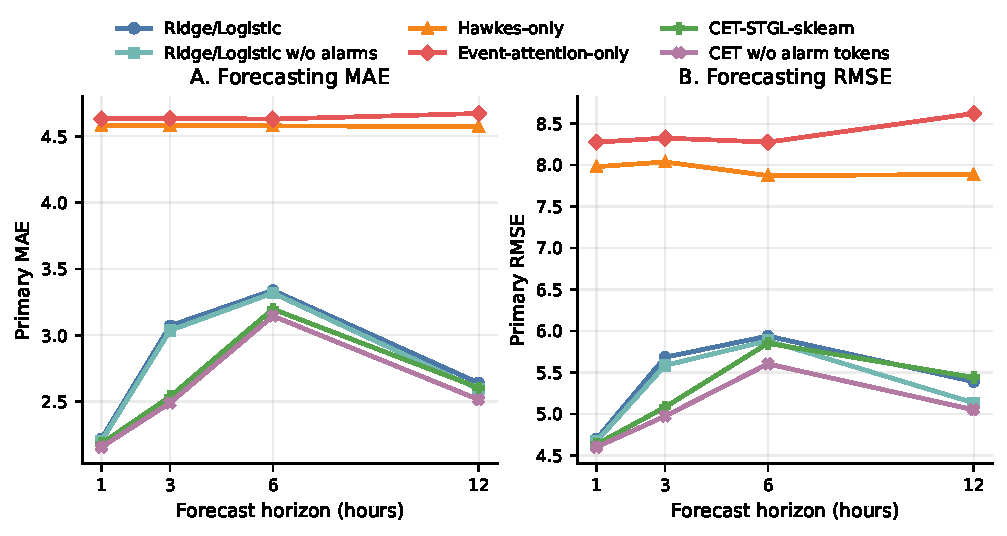
\includegraphics[width=\linewidth]{figures/Fig1_forecasting_vs_horizon.pdf}
    \caption{Primary-KPI forecasting error versus prediction horizon.}
    \label{fig:forecasting}
\end{figure}

\begin{figure}[t]
    \centering
    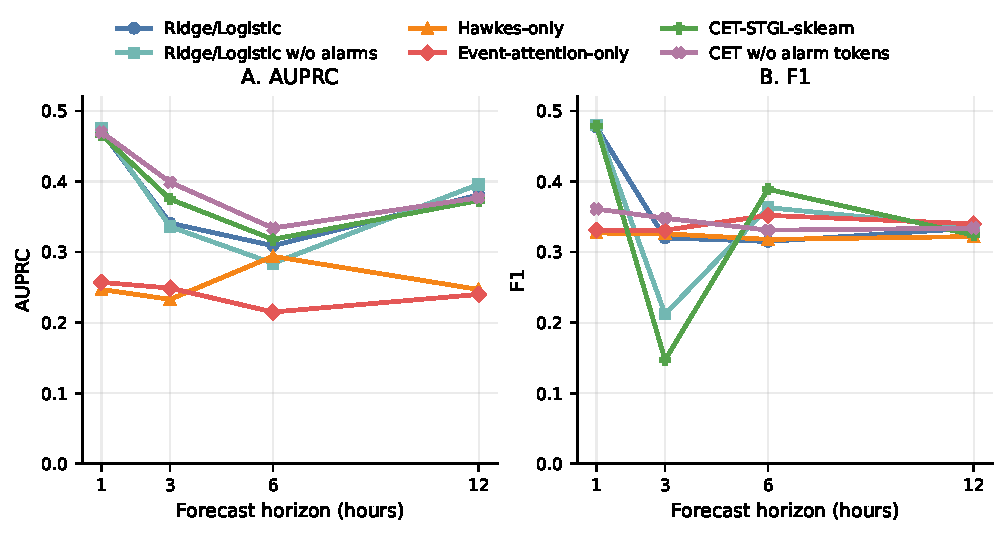
\includegraphics[width=\linewidth]{figures/Fig2_classification_comparison.pdf}
    \caption{KPI degradation classification performance versus prediction horizon.}
    \label{fig:classification}
\end{figure}

\begin{figure}[t]
    \centering
    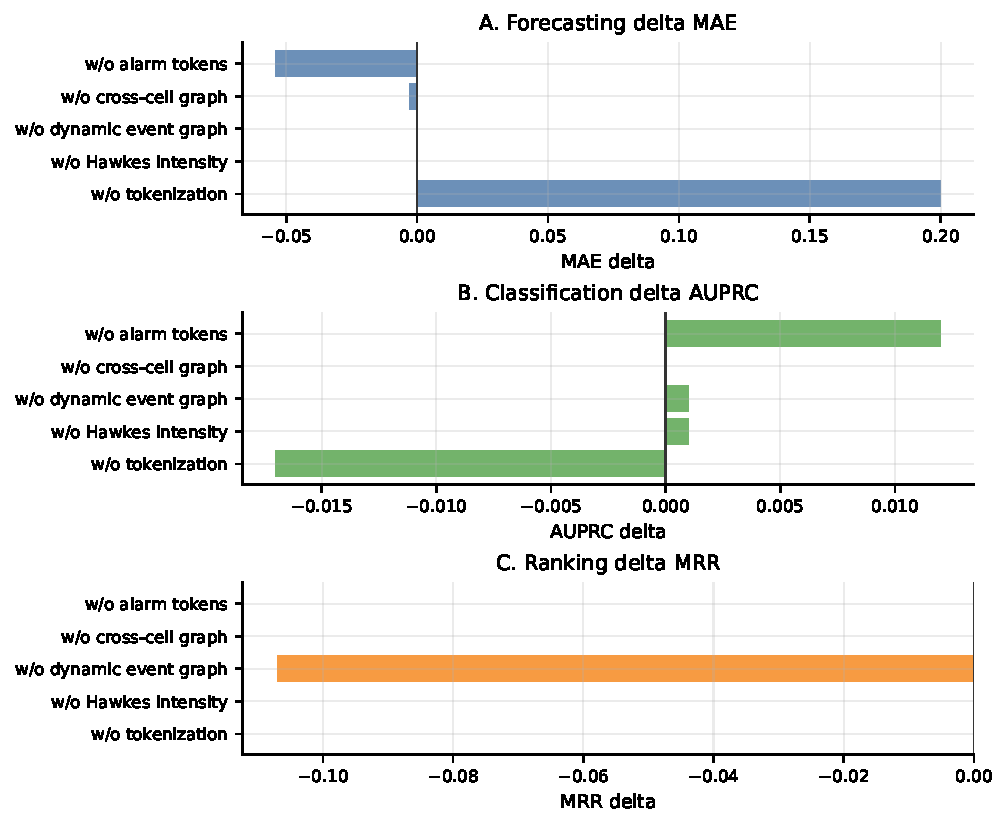
\includegraphics[width=\linewidth]{figures/Fig3_ablation_delta.pdf}
    \caption{Ablation deltas relative to CET-STGL-sklearn.}
    \label{fig:ablation}
\end{figure}

\begin{figure}[t]
    \centering
    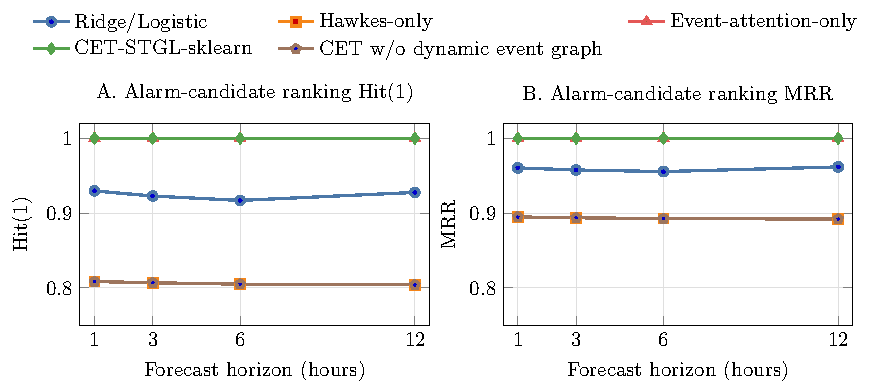
\includegraphics[width=\linewidth]{figures/Fig4_weak_ranking_comparison.pdf}
    \caption{Weak alarm-candidate ranking consistency versus prediction horizon.}
    \label{fig:ranking}
\end{figure}

\subsection{Limitations, Data Availability and Reproducibility}
\label{sec:limitations_reproducibility}
\label{sec:discussion_limitations}
\label{sec:data_availability}

The study is limited to the evaluated panel and weak labels. KPI histories and cell-time context carry most of the forecasting signal; alarm and inferred graph features yield limited, non-uniform aggregate gains. Weak alarm-candidate ranking is a proxy consistency check rather than expert-confirmed RCA, and the event influence graph captures observational association rather than estimated causal effects.

The chronological split tests future-time generalization within observed cells, not transfer to unseen regions, networks or deployments. End-to-end neural spatio-temporal graph evaluation is left to future work. Raw Huawei MBB records cannot be released because they include confidential operational KPI and alarm information. Code, sanitized schemas, synthetic validation data and experiment scripts are available at \url{https://github.com/DunLi-Tsinghua/cet-stgl-cellular-kpi}.

\section{Conclusion}
\label{sec:conclusion}
This paper presents CET-STGL, a causal-inspired event-token spatio-temporal framework for alarm-aware KPI degradation prediction in cellular networks. The main methodological contribution is a temporally admissible representation pipeline that organizes KPI histories, sparse alarm events, cell/time context, train-only event influence priors and inferred cross-cell context under a common reliability evaluation protocol. On anonymized Huawei MBB operations data, the evaluated lightweight instantiation is competitive with classical baselines on several primary-KPI forecasting metrics, while KPI-history and no-alarm variants remain strong. Alarm and graph features do not improve aggregate forecasting consistently in the evaluated slice, although alarm information remains relevant to the weak association-based prioritization protocol. The ranking task measures weak-label consistency rather than expert-confirmed fault localization. Future work should evaluate additional operational slices, incorporate verified topology where available, add expert incident annotations and test end-to-end neural spatio-temporal graph instantiations under the same protocol.


\clearpage
\appendix
\setcounter{table}{0}
\setcounter{figure}{0}
\renewcommand{\thetable}{A.\arabic{table}}
\renewcommand{\thefigure}{A.\arabic{figure}}

\section{Full Experimental Tables}

The main paper reports compact summary tables for readability. The appendix retains the full runnable model-by-horizon tables generated from the existing paper artifacts.

\subsection{Full Forecasting Results}
\begingroup
\scriptsize
\setlength{\tabcolsep}{3pt}
\begin{longtable}{@{}p{0.26\linewidth}rrrrrr@{}}
\caption{KPI forecasting results over runnable models and horizons.}
\label{tab:forecasting_results}\\
\toprule
Model & H & P-MAE & P-RMSE & P-MAPE & All-MAE & All-RMSE \\
\midrule
\endfirsthead
\toprule
Model & H & P-MAE & P-RMSE & P-MAPE & All-MAE & All-RMSE \\
\midrule
\endhead
CET w/o alarm tokens & 1 & 2.1569 & 4.6016 & 42.4111 & 30.1717 & 53.1923 \\
CET w/o cross-cell graph & 1 & 2.1791 & 4.6351 & 42.7362 & 31.1928 & 62.4168 \\
CET w/o dynamic event graph & 1 & 2.1831 & 4.6351 & 42.6425 & 31.2506 & 62.1414 \\
CET w/o Hawkes intensity & 1 & 2.1831 & 4.6351 & 42.6425 & 31.2506 & 62.1414 \\
CET w/o tokenization & 1 & 2.2244 & 4.7059 & 43.4812 & 31.6755 & 61.3319 \\
CET-STGL-sklearn & 1 & 2.1830 & 4.6351 & 42.6425 & 31.2510 & 62.1427 \\
Event-attention-only & 1 & 4.6305 & 8.2757 & 82.5194 & 163.9535 & 271.1688 \\
Hawkes-only & 1 & 4.5779 & 7.9814 & 82.2610 & 160.0211 & 227.2084 \\
Ridge/Logistic & 1 & 2.2191 & 4.6984 & 43.5993 & 31.4426 & 58.4626 \\
Ridge/Logistic w/o alarms & 1 & 2.2034 & 4.6712 & 43.3820 & 30.6931 & 53.7885 \\
CET w/o alarm tokens & 3 & 2.4904 & 4.9744 & 46.8069 & 39.4850 & 67.8885 \\
CET w/o cross-cell graph & 3 & 2.5354 & 5.0786 & 47.2707 & 42.1875 & 103.4692 \\
CET w/o dynamic event graph & 3 & 2.5368 & 5.0829 & 47.1621 & 42.1587 & 102.7291 \\
CET w/o Hawkes intensity & 3 & 2.5368 & 5.0829 & 47.1621 & 42.1587 & 102.7291 \\
CET w/o tokenization & 3 & 3.0549 & 5.6840 & 56.1056 & 50.7988 & 101.8653 \\
CET-STGL-sklearn & 3 & 2.5367 & 5.0829 & 47.1624 & 42.1585 & 102.7298 \\
Event-attention-only & 3 & 4.6346 & 8.3256 & 82.7764 & 164.6453 & 289.4013 \\
Hawkes-only & 3 & 4.5809 & 8.0385 & 82.5149 & 159.7122 & 227.2520 \\
Ridge/Logistic & 3 & 3.0709 & 5.6842 & 56.3815 & 50.7191 & 93.6261 \\
Ridge/Logistic w/o alarms & 3 & 3.0361 & 5.5858 & 56.0146 & 48.9354 & 78.7454 \\
CET w/o alarm tokens & 6 & 3.1447 & 5.6052 & 56.8431 & 50.7871 & 82.1649 \\
CET w/o cross-cell graph & 6 & 3.1904 & 5.8644 & 57.2840 & 54.4509 & 133.8707 \\
CET w/o dynamic event graph & 6 & 3.1970 & 5.8527 & 57.2636 & 54.4014 & 132.2650 \\
CET w/o Hawkes intensity & 6 & 3.1970 & 5.8527 & 57.2636 & 54.4014 & 132.2650 \\
CET w/o tokenization & 6 & 3.3631 & 6.0530 & 61.5916 & 65.4517 & 131.9830 \\
CET-STGL-sklearn & 6 & 3.1971 & 5.8527 & 57.2638 & 54.4004 & 132.2636 \\
Event-attention-only & 6 & 4.6287 & 8.2769 & 83.1170 & 164.8499 & 295.9310 \\
Hawkes-only & 6 & 4.5785 & 7.8735 & 82.8707 & 159.5017 & 225.5720 \\
Ridge/Logistic & 6 & 3.3380 & 5.9402 & 61.5904 & 65.1005 & 118.3171 \\
Ridge/Logistic w/o alarms & 6 & 3.3177 & 5.8838 & 61.2722 & 62.6208 & 97.5729 \\
CET w/o alarm tokens & 12 & 2.5147 & 5.0508 & 47.2830 & 42.0699 & 74.8636 \\
CET w/o cross-cell graph & 12 & 2.6040 & 5.4528 & 47.7833 & 46.2547 & 127.1682 \\
CET w/o dynamic event graph & 12 & 2.6041 & 5.4421 & 47.6820 & 46.4562 & 126.0803 \\
CET w/o Hawkes intensity & 12 & 2.6041 & 5.4421 & 47.6820 & 46.4562 & 126.0803 \\
CET w/o tokenization & 12 & 2.6796 & 5.5472 & 49.0619 & 47.8638 & 124.7888 \\
CET-STGL-sklearn & 12 & 2.6041 & 5.4421 & 47.6819 & 46.4562 & 126.0802 \\
Event-attention-only & 12 & 4.6714 & 8.6216 & 83.3406 & 164.9266 & 287.0291 \\
Hawkes-only & 12 & 4.5719 & 7.8884 & 83.0608 & 160.6519 & 238.1456 \\
Ridge/Logistic & 12 & 2.6400 & 5.3913 & 49.1403 & 47.3654 & 122.6165 \\
Ridge/Logistic w/o alarms & 12 & 2.5928 & 5.1347 & 48.8058 & 43.2913 & 76.8817 \\
\bottomrule
\end{longtable}
\endgroup
\noindent\footnotesize{Note. Forecasting labels are real future KPI values. MAPE uses denominator floor $\max(|y|,1.0)$. Neural baselines are not run because the PyTorch backend is unavailable. Root-cause ranking is weak-label/proxy consistency, not expert-confirmed root cause. The event graph is causal-inspired / causal discovery-based, not confirmed causality.}


\subsection{Full Weak Degradation Classification Results}
\begingroup
\scriptsize
\setlength{\tabcolsep}{3pt}
\begin{longtable}{@{}p{0.26\linewidth}rrrrrr@{}}
\caption{Weak KPI degradation classification results.}
\label{tab:classification_results}\\
\toprule
Model & H & AUPRC & F1 & Prec. & Recall & AUROC \\
\midrule
\endfirsthead
\toprule
Model & H & AUPRC & F1 & Prec. & Recall & AUROC \\
\midrule
\endhead
CET-STGL without alarm tokens & 1 & 0.4702 & 0.3609 & 0.2215 & 0.9746 & 0.7975 \\
CET-STGL without cross-cell graph & 1 & 0.4482 & 0.3980 & 0.5244 & 0.3207 & 0.7827 \\
CET-STGL without dynamic event graph & 1 & 0.4662 & 0.4784 & 0.3948 & 0.6070 & 0.7943 \\
CET-STGL without Hawkes intensity & 1 & 0.4662 & 0.4785 & 0.3947 & 0.6074 & 0.7944 \\
CET-STGL without tokenization & 1 & 0.4578 & 0.4583 & 0.4634 & 0.4534 & 0.7892 \\
CET-STGL-sklearn & 1 & 0.4663 & 0.4787 & 0.3949 & 0.6078 & 0.7944 \\
Event-attention-only & 1 & 0.2573 & 0.3310 & 0.2257 & 0.6201 & 0.6358 \\
Hawkes-only & 1 & 0.2465 & 0.3274 & 0.2181 & 0.6562 & 0.6314 \\
LSTM & 1 & 0.4477 & 0.4042 & 0.2769 & 0.7479 & 0.7553 \\
TCN & 1 & 0.2699 & 0.3891 & 0.2773 & 0.6518 & 0.6846 \\
Ridge/Logistic & 1 & 0.4709 & 0.4774 & 0.4182 & 0.5563 & 0.7946 \\
Ridge/Logistic without alarms & 1 & 0.4756 & 0.4801 & 0.3956 & 0.6104 & 0.7971 \\
CET-STGL without alarm tokens & 3 & 0.3990 & 0.3481 & 0.5197 & 0.2617 & 0.7587 \\
CET-STGL without cross-cell graph & 3 & 0.3870 & 0.4010 & 0.2700 & 0.7787 & 0.7527 \\
CET-STGL without dynamic event graph & 3 & 0.3760 & 0.1475 & 0.5751 & 0.0846 & 0.7430 \\
CET-STGL without Hawkes intensity & 3 & 0.3759 & 0.1476 & 0.5780 & 0.0846 & 0.7429 \\
CET-STGL without tokenization & 3 & 0.3419 & 0.3121 & 0.1849 & 0.9985 & 0.7236 \\
CET-STGL-sklearn & 3 & 0.3752 & 0.1468 & 0.5696 & 0.0842 & 0.7427 \\
Event-attention-only & 3 & 0.2494 & 0.3310 & 0.2183 & 0.6836 & 0.6328 \\
Hawkes-only & 3 & 0.2331 & 0.3265 & 0.2181 & 0.6492 & 0.6230 \\
LSTM & 3 & 0.3703 & 0.3899 & 0.2678 & 0.7166 & 0.7207 \\
TCN & 3 & 0.2198 & 0.3340 & 0.2260 & 0.6402 & 0.6193 \\
Ridge/Logistic & 3 & 0.3409 & 0.3201 & 0.1907 & 0.9959 & 0.7231 \\
Ridge/Logistic without alarms & 3 & 0.3365 & 0.2118 & 0.4454 & 0.1389 & 0.7256 \\
CET-STGL without alarm tokens & 6 & 0.3344 & 0.3313 & 0.1996 & 0.9750 & 0.7167 \\
CET-STGL without cross-cell graph & 6 & 0.3195 & 0.3318 & 0.1997 & 0.9792 & 0.7178 \\
CET-STGL without dynamic event graph & 6 & 0.3203 & 0.3894 & 0.2853 & 0.6129 & 0.7131 \\
CET-STGL without Hawkes intensity & 6 & 0.3203 & 0.3892 & 0.2849 & 0.6136 & 0.7131 \\
CET-STGL without tokenization & 6 & 0.3026 & 0.3033 & 0.3729 & 0.2556 & 0.6842 \\
CET-STGL-sklearn & 6 & 0.3181 & 0.3887 & 0.2835 & 0.6181 & 0.7127 \\
Event-attention-only & 6 & 0.2146 & 0.3523 & 0.2455 & 0.6234 & 0.6165 \\
Hawkes-only & 6 & 0.2940 & 0.3183 & 0.2152 & 0.6113 & 0.6326 \\
LSTM & 6 & 0.3505 & 0.3678 & 0.2462 & 0.7270 & 0.7024 \\
TCN & 6 & 0.1991 & 0.3129 & 0.2111 & 0.6045 & 0.5831 \\
Ridge/Logistic & 6 & 0.3087 & 0.3152 & 0.4025 & 0.2590 & 0.6909 \\
Ridge/Logistic without alarms & 6 & 0.2840 & 0.3625 & 0.2448 & 0.6983 & 0.6830 \\
CET-STGL without alarm tokens & 12 & 0.3769 & 0.3337 & 0.2007 & 0.9885 & 0.7526 \\
CET-STGL without cross-cell graph & 12 & 0.3777 & 0.3213 & 0.1915 & 0.9981 & 0.7499 \\
CET-STGL without dynamic event graph & 12 & 0.3728 & 0.3243 & 0.1937 & 0.9966 & 0.7463 \\
CET-STGL without Hawkes intensity & 12 & 0.3729 & 0.3243 & 0.1937 & 0.9966 & 0.7463 \\
CET-STGL without tokenization & 12 & 0.3641 & 0.3633 & 0.4503 & 0.3045 & 0.7382 \\
CET-STGL-sklearn & 12 & 0.3732 & 0.3240 & 0.1934 & 0.9966 & 0.7465 \\
Event-attention-only & 12 & 0.2405 & 0.3396 & 0.2383 & 0.5904 & 0.6332 \\
Hawkes-only & 12 & 0.2467 & 0.3221 & 0.2190 & 0.6083 & 0.6107 \\
LSTM & 12 & 0.3801 & 0.3763 & 0.2622 & 0.6664 & 0.7101 \\
TCN & 12 & 0.1896 & 0.2885 & 0.1958 & 0.5480 & 0.5695 \\
Ridge/Logistic & 12 & 0.3806 & 0.3339 & 0.2011 & 0.9828 & 0.7413 \\
Ridge/Logistic without alarms & 12 & 0.3959 & 0.3348 & 0.2018 & 0.9828 & 0.7420 \\
\bottomrule
\end{longtable}
\endgroup


\subsection{Full Weak Ranking Results}
\begingroup
\scriptsize
\setlength{\tabcolsep}{3pt}
\begin{longtable}{@{}p{0.24\linewidth}rrrrrrr@{}}
\caption{Weak alarm-candidate ranking consistency.}
\label{tab:weak_ranking_results}\\
\toprule
Model & H & N & $\mathrm{Hit}(1)$ & $\mathrm{Hit}(3)$ & $\mathrm{Hit}(5)$ & MRR & $\mathrm{nDCG}(5)$ \\
\midrule
\endfirsthead
\toprule
Model & H & N & $\mathrm{Hit}(1)$ & $\mathrm{Hit}(3)$ & $\mathrm{Hit}(5)$ & MRR & $\mathrm{nDCG}(5)$ \\
\midrule
\endhead
CET-STGL without alarm tokens & 1 & 0 &  &  &  &  &  \\
CET-STGL without cross-cell graph & 1 & 2682 & 1.0000 & 1.0000 & 1.0000 & 1.0000 & 1.0000 \\
CET-STGL without dynamic event graph & 1 & 2682 & 0.8084 & 0.9952 & 0.9959 & 0.8948 & 0.9204 \\
CET-STGL without Hawkes intensity & 1 & 611 & 1.0000 & 1.0000 & 1.0000 & 1.0000 & 1.0000 \\
CET-STGL without tokenization & 1 & 2682 & 1.0000 & 1.0000 & 1.0000 & 1.0000 & 1.0000 \\
CET-STGL-sklearn & 1 & 2682 & 1.0000 & 1.0000 & 1.0000 & 1.0000 & 1.0000 \\
Event-attention-only & 1 & 611 & 1.0000 & 1.0000 & 1.0000 & 1.0000 & 1.0000 \\
Hawkes-only & 1 & 2682 & 0.8084 & 0.9952 & 0.9959 & 0.8948 & 0.9204 \\
Ridge/Logistic & 1 & 611 & 0.9296 & 1.0000 & 1.0000 & 0.9604 & 0.9706 \\
Ridge/Logistic without alarms & 1 & 0 &  &  &  &  &  \\
CET-STGL without alarm tokens & 3 & 0 &  &  &  &  &  \\
CET-STGL without cross-cell graph & 3 & 2671 & 1.0000 & 1.0000 & 1.0000 & 1.0000 & 1.0000 \\
CET-STGL without dynamic event graph & 3 & 2671 & 0.8068 & 0.9944 & 0.9951 & 0.8937 & 0.9193 \\
CET-STGL without Hawkes intensity & 3 & 609 & 1.0000 & 1.0000 & 1.0000 & 1.0000 & 1.0000 \\
CET-STGL without tokenization & 3 & 2671 & 1.0000 & 1.0000 & 1.0000 & 1.0000 & 1.0000 \\
CET-STGL-sklearn & 3 & 2671 & 1.0000 & 1.0000 & 1.0000 & 1.0000 & 1.0000 \\
Event-attention-only & 3 & 609 & 1.0000 & 1.0000 & 1.0000 & 1.0000 & 1.0000 \\
Hawkes-only & 3 & 2671 & 0.8068 & 0.9944 & 0.9951 & 0.8937 & 0.9193 \\
Ridge/Logistic & 3 & 609 & 0.9228 & 1.0000 & 1.0000 & 0.9576 & 0.9685 \\
Ridge/Logistic without alarms & 3 & 0 &  &  &  &  &  \\
CET-STGL without alarm tokens & 6 & 0 &  &  &  &  &  \\
CET-STGL without cross-cell graph & 6 & 2645 & 1.0000 & 1.0000 & 1.0000 & 1.0000 & 1.0000 \\
CET-STGL without dynamic event graph & 6 & 2645 & 0.8049 & 0.9940 & 0.9947 & 0.8926 & 0.9183 \\
CET-STGL without Hawkes intensity & 6 & 614 & 1.0000 & 1.0000 & 1.0000 & 1.0000 & 1.0000 \\
CET-STGL without tokenization & 6 & 2645 & 1.0000 & 1.0000 & 1.0000 & 1.0000 & 1.0000 \\
CET-STGL-sklearn & 6 & 2645 & 1.0000 & 1.0000 & 1.0000 & 1.0000 & 1.0000 \\
Event-attention-only & 6 & 614 & 1.0000 & 1.0000 & 1.0000 & 1.0000 & 1.0000 \\
Hawkes-only & 6 & 2645 & 0.8049 & 0.9940 & 0.9947 & 0.8926 & 0.9183 \\
Ridge/Logistic & 6 & 614 & 0.9169 & 1.0000 & 1.0000 & 0.9555 & 0.9670 \\
Ridge/Logistic without alarms & 6 & 0 &  &  &  &  &  \\
CET-STGL without alarm tokens & 12 & 0 &  &  &  &  &  \\
CET-STGL without cross-cell graph & 12 & 2617 & 1.0000 & 1.0000 & 1.0000 & 1.0000 & 1.0000 \\
CET-STGL without dynamic event graph & 12 & 2617 & 0.8040 & 0.9935 & 0.9943 & 0.8920 & 0.9177 \\
CET-STGL without Hawkes intensity & 12 & 649 & 1.0000 & 1.0000 & 1.0000 & 1.0000 & 1.0000 \\
CET-STGL without tokenization & 12 & 2617 & 1.0000 & 1.0000 & 1.0000 & 1.0000 & 1.0000 \\
CET-STGL-sklearn & 12 & 2617 & 1.0000 & 1.0000 & 1.0000 & 1.0000 & 1.0000 \\
Event-attention-only & 12 & 649 & 1.0000 & 1.0000 & 1.0000 & 1.0000 & 1.0000 \\
Hawkes-only & 12 & 2617 & 0.8040 & 0.9935 & 0.9943 & 0.8920 & 0.9177 \\
Ridge/Logistic & 12 & 649 & 0.9276 & 1.0000 & 1.0000 & 0.9617 & 0.9717 \\
Ridge/Logistic without alarms & 12 & 0 &  &  &  &  &  \\
\bottomrule
\end{longtable}
\endgroup


\subsection{Full Ablation Delta Table}
\begingroup
\scriptsize
\setlength{\tabcolsep}{3pt}
\begin{longtable}{@{}p{0.24\linewidth}p{0.19\linewidth}rrrr@{}}
\caption{Ablation deltas relative to CET-STGL-sklearn.}
\label{tab:ablation_delta}\\
\toprule
Ablation row & Removed & H & $\Delta$ P-MAE & $\Delta$ AUPRC & $\Delta$ MRR \\
\midrule
\endfirsthead
\toprule
Ablation row & Removed & H & $\Delta$ P-MAE & $\Delta$ AUPRC & $\Delta$ MRR \\
\midrule
\endhead
CET-STGL without alarm tokens & \makecell[l]{no\_alarm} & 1 & -0.0262 & 0.0039 &  \\
CET-STGL without alarm tokens & \makecell[l]{no\_alarm} & 3 & -0.0463 & 0.0238 &  \\
CET-STGL without alarm tokens & \makecell[l]{no\_alarm} & 6 & -0.0524 & 0.0162 &  \\
CET-STGL without alarm tokens & \makecell[l]{no\_alarm} & 12 & -0.0893 & 0.0037 &  \\
CET-STGL without cross-cell graph & \makecell[l]{no\_cross\\cell\_graph} & 1 & -0.0039 & -0.0181 & 0.0000 \\
CET-STGL without cross-cell graph & \makecell[l]{no\_cross\\cell\_graph} & 3 & -0.0014 & 0.0118 & 0.0000 \\
CET-STGL without cross-cell graph & \makecell[l]{no\_cross\\cell\_graph} & 6 & -0.0066 & 0.0014 & 0.0000 \\
CET-STGL without cross-cell graph & \makecell[l]{no\_cross\\cell\_graph} & 12 & -0.0001 & 0.0045 & 0.0000 \\
CET-STGL without dynamic event graph & \makecell[l]{no\_dynamic\\graph} & 1 & 0.0001 & -0.0001 & -0.1052 \\
CET-STGL without dynamic event graph & \makecell[l]{no\_dynamic\\graph} & 3 & 0.0000 & 0.0007 & -0.1063 \\
CET-STGL without dynamic event graph & \makecell[l]{no\_dynamic\\graph} & 6 & -0.0001 & 0.0022 & -0.1074 \\
CET-STGL without dynamic event graph & \makecell[l]{no\_dynamic\\graph} & 12 & -0.0000 & -0.0004 & -0.1080 \\
CET-STGL without Hawkes intensity & \makecell[l]{no\_hawkes\\intensity} & 1 & 0.0001 & -0.0001 & 0.0000 \\
CET-STGL without Hawkes intensity & \makecell[l]{no\_hawkes\\intensity} & 3 & 0.0000 & 0.0007 & 0.0000 \\
CET-STGL without Hawkes intensity & \makecell[l]{no\_hawkes\\intensity} & 6 & -0.0001 & 0.0022 & 0.0000 \\
CET-STGL without Hawkes intensity & \makecell[l]{no\_hawkes\\intensity} & 12 & -0.0000 & -0.0003 & 0.0000 \\
CET-STGL without tokenization & \makecell[l]{no\_tokenization} & 1 & 0.0414 & -0.0085 & 0.0000 \\
CET-STGL without tokenization & \makecell[l]{no\_tokenization} & 3 & 0.5181 & -0.0333 & 0.0000 \\
CET-STGL without tokenization & \makecell[l]{no\_tokenization} & 6 & 0.1660 & -0.0155 & 0.0000 \\
CET-STGL without tokenization & \makecell[l]{no\_tokenization} & 12 & 0.0755 & -0.0091 & 0.0000 \\
\bottomrule
\end{longtable}
\endgroup


\clearpage
\section{Nomenclature}
% Reset table counter and update prefix for Appendix B
\setcounter{table}{0}
\renewcommand{\thetable}{B.\arabic{table}}
\begingroup
\scriptsize
\setlength{\tabcolsep}{3pt}
\begin{longtable}{@{}lp{0.8\linewidth}@{}}
\caption{Nomenclature of Acronyms and Symbols.}
\label{tab:nomenclature}\\
\toprule
\textbf{Item} & \textbf{Description} \\
\midrule
\endfirsthead
\toprule
\textbf{Item} & \textbf{Description} \\
\midrule
\endhead

\multicolumn{2}{@{}l}{\textbf{Acronyms}} \\
\midrule
AIOps & Artificial Intelligence for IT Operations \\
AUPRC & Area Under the Precision-Recall Curve \\
AUROC & Area Under the Receiver Operating Characteristic Curve \\
CET-STGL & Causal-Inspired Event-Token Spatio-Temporal Framework \\
KPI & Key Performance Indicator \\
MAE & Mean Absolute Error \\
MAPE & Mean Absolute Percentage Error \\
MBB & Mobile Broadband \\
MRR & Mean Reciprocal Rank \\
nDCG & Normalized Discounted Cumulative Gain \\
O-RAN & Open Radio Access Network \\
RCA & Root-Cause Analysis \\
RMSE & Root Mean Square Error \\

\midrule
\multicolumn{2}{@{}l}{\textbf{Symbols}} \\
\midrule
$\mathcal{C}$ & Set of evaluated cellular sites \\
$c, t$ & Indices for cell entity and hourly timestamp \\
$h$ & Forecasting horizon in hours ($h \in \{1, 3, 6, 12\}$) \\
$L$ & Lookback window length \\
$\mathbf{x}_{c,t}$ & KPI and business counter vector at cell $c$, time $t$ \\
$\mathbf{a}_{c,t}$ & Alarm and fault vector at cell $c$, time $t$ \\
$\mathcal{W}_{c,t}$ & Historical lookback window for a given cell and time \\
$M, A$ & Dimensionality of KPI vector and alarm vector, respectively \\
$f_h, g_h, r_h$ & Mapping functions for forecasting, classification, and ranking tasks \\
$\hat{\mathbf{x}}_{c,t+h}$ & Predicted KPI vector at horizon $h$ \\
$y_{c,t+h}, \hat{y}_{c,t+h}$ & Ground-truth weak binary degradation indicator and predicted probability \\
$\mathcal{A}_{c,t}$ & Set of candidate alarm types for ranking \\
$s_h(a,c,t)$ & Ranking score assigned to alarm candidate $a$ \\
$\phi^{\mathrm{kpi}}_{c,t,p,m}$ & Extracted patch-based feature summary for KPI $m$ \\
$\lambda_a(c,t)$ & Decayed event intensity for alarm type $a$ \\
$\eta$ & Fixed decay scale for event intensity \\
$\mathrm{lift}_h(a)$ & Train-only event influence prior (lagged lift) for alarm $a$ \\
$P_{\mathrm{train}}$ & Probability estimated within the training set \\
$G_{\mathrm{cell}}$ & Inferred cross-cell statistical context graph \\
$E$ & Edges within the cross-cell graph $G_{\mathrm{cell}}$ \\
\bottomrule
\end{longtable}
\endgroup


\section{Data Availability and Reproducibility}

The underlying Huawei MBB operational records are anonymized enterprise data and cannot be publicly released because they contain confidential network performance and alarm information. To support reproducibility within these restrictions, the project repository provides the source code, sanitized schema, synthetic examples and artifacts used to generate the manuscript tables and figures. Exact metric reproduction requires authorized access to the raw operational records and the chronological train-only fitting protocol described in Section~\ref{sec:data_protocol}.


\bibliographystyle{elsarticle-num}
\bibliography{refs}

\end{document}
